\chapter{Theoretische Grundlagen}
In diesem Kapitel wird in die benutzen Konzepte eingeführt.

\section{Energy Harvesting}
\glqq Mit Energy Harvesting ... wird die Gewinnung von elektrischer Energie in kleinen Mengen aus dem Umfeld elektronischer Geräte für deren Betrieb bezeichnet.\grqq \cite{harvesting}


Bekannte Methoden sind Thermogeneratoren, die aus Umgebungswärme Energie gewinnen, passive RFID-Tags, die aus der elektromagnetischen Strahlung Energie gewinnen und der piezoelektrische Effekt, der mechanischen Druck in elektrische Spannung umwandelt. 

In dieser Bachelorarbeit wird Energie über Bewegungsinduktion gewonnen. Die nachfolgenden Erklärungen stammen aus \cite{PA_bicycle} S.8.  
\subsection*{Bewegungsindktion}

Befindet sich eine Spule in einem \textit{dynamischen} \glqq Magnetfeld\grqq, wird in der Spule eine Spannung induziert. Dies sieht man in der Formel (\ref{Formel_induzSpannung}).

\begin{equation}
    U_{ind}=-\frac{d}{dt}\intop A\,dB \ \label{Formel_induzSpannung} 
\end{equation}

Der magnetische Fluss $B$ durch die Fläche einer Spule $A$ ist gleich dem magnetischen Fluss $\phi$. Hat die Spule mehrere Wicklungen $N$, so verstärkt sich der magnetische Fluss proportional. 

 
\begin{equation}
    \frac{d}{dt} \int A\,dB=\phi\cdot N\
\end{equation}

Verläuft der \textbf{magnetische Flus???}s $\phi$ senkrecht zur Fläche der Spule $A$ kann das Integral durch eine Multiplikation ersetzt werden (siehe Formel\label{Formel_senkrecht}). 
 
\begin{equation}
    \frac{d}{dt} \int A\,\perp\, dB=\frac{d}{dt}\int \phi\cdot N=B\cdot A\cdot N\ \label{Formel_senkrecht} 
\end{equation} 
  
 
In diesem Fall berechnet sich die induzierte Spannung in einer Spule vereinfacht mit
\begin{equation}
    U_{ind}= - N \cdot A \cdot B
\end{equation}

Das dynamische Magnetfeld wird durch das Bewegen, oder im Fall eines Fahrrads einem Vorbeiziehen, eines Magneten an einer fix verankerten Spule erzeugt.
Die produzierte Spannung hängt von drei Kriterien ab:

Eine induzierte Spannung wird somit durch folgende vier Faktoren beinflusst:
\begin{enumerate}
    \item die eingeschlossene Fläche $A$ der Spule    
    \item die \textbf{magnetische Flussdichte???} des Magneten $B$ 
    \item die Anzahl Windungen $N$ der Spule und
    \item die Bewegungsgeschwindigkeit $v$ des Magneten, welche Einfluss auf $dt$ hat
\end{enumerate}

(Für die Schaltungsoptimierung sind die ersten drei Punkte relevant.)

\section{Energy Management für die gewonnene Energie}
Was wir machen: HRV Energie nicht direkt in sensortag, sondern in LTS speichern.

In der Bachelorarbeit ist bei der Umsetzung des Enerergymanagements der Chip EM8500 vorgegeben. Dieser IC ist von EM Microelectronics aus Marin (NE) entwickelt. %( Alternative Powermanagementsysteme sind z. B. : Booster TI, Analog Devices, E-Beas.)


Energy Management bezeichnet das Regeln von Energiezuständen, damit ein Optimum an Leistung aus einer Quelle bezogen werden kann.


%The EM8500 is an autonomous power management system able to manage power domains, power sources and storage elements \cite{datasheet_EM85}, p. 11.

Zu diesem Chip ist das Evaluation-Board EMEVB8500 (im Text mit EVB abgekürzt) entwickelt, welches das Aufsetzen eines energieoptimierten Systems unterstützt. 


\subsection{Regelung des optimalen Leistungsbezugs}

Generell MPP beschreiben, nicht EM MPP
Widerstandskurve als Graphik nehmen
MPP ist wie Leistungsanpasung

Wichtigster Punkt in der Energieoptimierung ist das Maximum aus der produzierten Energie herauszuholen. Die maximale Leistung ergibt sich beim MaximumPowerPoints (MPP), dem Punkte, an denen am effizientesten Leistung bezogen werden kann. 
Das EVB versucht die Quelle stets in der Nähe dieses Optimums zu betreiben. Dies geschieht über eine Innenwiderstand-Regelung, sodass die Eingangsleistung möglichst dem MPP entspricht.

Zweite Aufgabe beim Energiemanagement ist eine konstante Eingangsspannungen zu erzwingen. Das System kontrolliert periodisch den aktuellen (unregulierten) Spannungswert der Harvestingquelle. Hat sich der Wert mehr als 37 mV gegenüber der zur Zeit aktuellen Regelspannung geändert, wird der neue Wert als Spannungsreferenz zum Regeln genommen. Die Abbildung \ref{RegelungSpannung} zeigt das Anpassen der Spannungslevel alle s. Die periodischen Kontrollmessungen alle 8 s verursachen kurze Spannungsspitzen. Diese entstehen bei der Kurzschlussmessung, für den akutellen Stromwert.


\begin{figure}    
    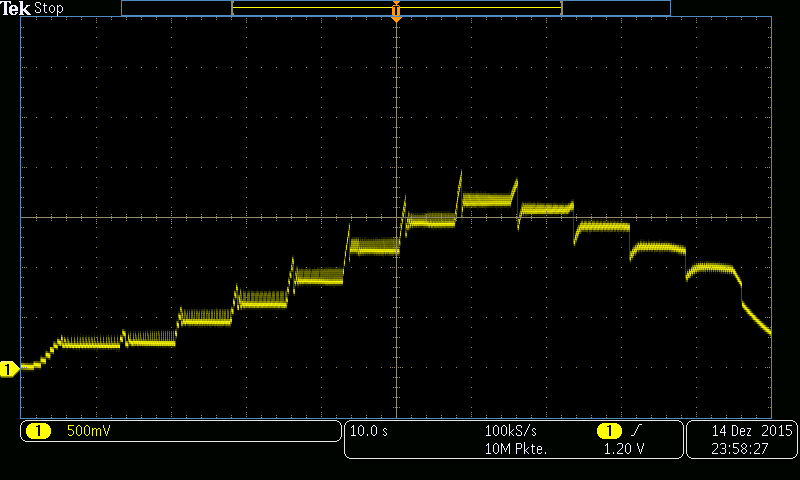
\includegraphics[width=15cm]{2TheoretischeGrundlagen/imag/RegelungVHRV.png}
    \caption{Spannungswerte Modell der Machbarkeitsstudie}\label{RegelungSpannung} 
\end{figure}

Entsprechen die Konfigurationen auf dem EVB nicht dem Verhalten der Eingangsquelle, so entstehen keine konstanten Spannungswerte an der Harvestingquelle, was Abbildung \ref{falscheRegelung} zeigt.

\begin{figure}
    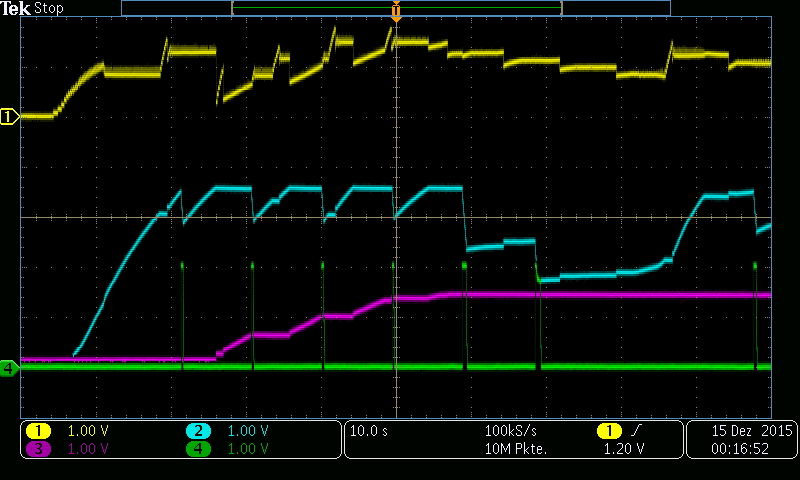
\includegraphics[width=15cm]{2TheoretischeGrundlagen/imag/falscheRegelung.png}
    \caption{Spannungswerte Modell der Machbarkeitsstudie}\label{falscheRegelung} 
\end{figure}

Dritter Punkt ist der Aufbau von Energiespeichern. Diese sollen so viel Energie speichern, wie eine gewisse Aktion braucht. Das Energiemanagmenet kennt für jede Aktion den Energieverbrauch und löst, bei genügend Speicherenergie eine Aktion laufen (siehe Berechnung der Kondensatoren).

Das Berechnen der Schwellwerte und der Kondensatoren detaillierter in Kapitel XXXXS.






\subsubsection{Energiestände kontrollieren}

Sobald genügend Startenergie bereit steht, wacht der EM8500-Chips auf. Neben dem Setzen der Konfigurationen aus dem EPROM kontrolliert der Chip als erstes den aktuellen Speicherzustand der angeschlossenen Speicher.

Die Engeriequelle wie auch die angeschlossenen Speicher haben eigene Pins, die ihren Zustand übermitteln\cite{datasheet_EM85}, p.11. 

Kommunikationsschema ? 

% -------------------------------------------------------
\section{Low Power Microcontroller von Texas Instruments}
- Zeichnen des Init, sleep, Aufwachen

Zur Verwaltung der gegebenen Energie ist der Microcontroller gegeben. Es handelt sich um einen Cortex M3, der sich auf dem Sensortag von Texas Instruments befindet. Die zentralen Eigenschaften dieses Boards und die Funktionsblöcke befindet sich im Anhang \ref{anhang_sensortag}.

\subsection{Fähigkeiten eines Low Power Microcontrollers}
  
Low Power Microcontroller können Gebiete des Prozessors oder von Periopherieelementen temporär ausschalten. Das System befindet sich im Standby Modus. Nur die für die Applikation unabdingbaren Aktivitäten laufen mit niederstem Takt weiter. Über Interrupts können einzelne Bereich aufgeweckt werden, die ihre Aktionen ausführen und danach geht das System wieder in den Standby Modus.

Bild: Energie-Langzeitmessung BLE versenden
Beschriften mit aktiv und standby modus

Zu den unabdingbaren Aktivitäten eines laufenden Microcontrollers gehört das Refreshen (Neuladen) der Register mit den Systemeinstellungen. Diese Refreshing-Peaks sieht man im Standby Modus.



\section{Aufsetzen des Low Power Microcontrollers}
%Üblicherweise wird das RTOS-Betriebssystem von TI für Low Power Applikationen benutzt. 
(Die Low-Power Programmbeispiele von TI basieren auf RTOS, ebenso die Dokumentation zu Low Power Applikationen, was zu viel Energie verbraucht (korrekt, wie belegen?). )

Konfiguration der CPU (system.h, config.h)
Einstellungen Active Mode: Sensoren, Wireless Processor, SPI-Kommunikation

Einstellungen sleep Mode: Abstellen

PowerDomain ausschalten
Clk

GPiO Konfigurieren (gpio.h, board.h)
Event anstelle von Interrupt
Synchronisation
timer, oder systick oder GPiO signal. Wake up

Aktivitäten aufsetzen







\section{Bluetooth Low Energy}

Unterschied zu Bluetooth

Spezifikationen





